\documentclass[11pt]{amsart}
\usepackage{amsmath,amssymb,amsthm,mathtools,mathrsfs}
\usepackage[margin=1.08in]{geometry}
\usepackage{booktabs}
\usepackage{array}
\usepackage{longtable}
\usepackage{tabularx}
\usepackage[table]{xcolor}
\usepackage{tikz}
\usepackage[hypertexnames=false]{hyperref}
\hypersetup{hidelinks}
\usepackage[final,expansion=false]{microtype}
\usepackage{url}
\setlength{\parskip}{4pt plus 1pt}
\emergencystretch=2.5em

\newtheorem{theorem}{Theorem}[section]
\newtheorem{proposition}[theorem]{Proposition}
\newtheorem{lemma}[theorem]{Lemma}
\newtheorem{corollary}[theorem]{Corollary}
\theoremstyle{definition}
\newtheorem{definition}[theorem]{Definition}
\newtheorem{problem}[theorem]{Problem}
\newtheorem{requirement}[theorem]{Requirement}
\theoremstyle{remark}
\newtheorem{remark}[theorem]{Remark}

\newcommand{\C}{\mathbb C}
\newcommand{\R}{\mathbb R}
\newcommand{\N}{\mathbb N}
\newcommand{\Z}{\mathbb Z}
\newcommand{\Q}{\mathbb Q}
\newcommand{\Rel}{\operatorname{Re}}
\newcommand{\Iml}{\operatorname{Im}}
\newcommand{\supp}{\operatorname{supp}}
\newcommand{\PT}{\mathcal P_T}
\newcommand{\IT}{I_T}
\newcommand{\lamA}{\lambda_{\mathrm A}(T)}
\newcommand{\lamW}{\lambda^{\mathrm W}_T}
\newcommand{\sT}{\sigma_T}
\newcommand{\Fh}{\widehat F}
\newcommand{\NT}{\mathcal N_T}
\newcommand{\mT}{\mathfrak m_T}
\newcommand{\eT}{\mathfrak e_T}
\newcommand{\Aev}{\mathfrak A_{\mathrm{ev}}}
\newcommand{\chiev}{\chi_{\mathrm{ev}}}
\newcommand{\Leb}{\mathrm{Leb}}
\newcommand{\cL}{\mathscr L}
\newcolumntype{Y}{>{\raggedright\arraybackslash}X}
\newcolumntype{L}[1]{>{\raggedright\arraybackslash}p{#1}}

\definecolor{cDead}{RGB}{70,72,82}
\definecolor{cRes}{RGB}{214,120,74}
\definecolor{cOpen}{RGB}{120,178,214}

\begin{document}

\title[A map of the routes to Weil positivity]
{A Map of the Routes to Weil Positivity on Finite Windows:\\
Barriers, Falsifiers, and the Open Inequality}

\author{David Alejandro Trejo Pizzo}
\thanks{Independent Researcher. \texttt{dtrejopizzo@gmail.com}.}

\date{\today}

\begin{abstract}
Let $\mathfrak a_T$ be the truncated Weil form on $L^2(-T,T)$ and $\lambda_{\mathrm A}(T)$ its bottom on the
subspace $\mathcal P_T$ where both Tate moments vanish. Window positivity, $\lambda_{\mathrm A}(T)\ge0$ for every
$T>0$, is certified for $T\le\frac12\log5$ in ball arithmetic and, by a cited certificate whose computational part
has been reproduced, for $T\le\frac12\log15$; beyond that it is open. This paper is a map of the arguments that
have been tried for the remaining windows, about seventeen hundred in all, and of the exact place where each one
fails. We first describe the shape of the sign: the archimedean form has about $4T$ negative directions, the prime
comb must cancel all of them but one, the remaining one is the polar direction, and in the Dirichlet sine basis the
comb is an explicit Toeplitz-plus-Hankel matrix in which this cancellation is a finite statement. We then state
the barrier theorems, each a theorem about a declared class of arguments proved by an explicit falsifier, list the
certified falsifiers, and derive the requirements they impose on any proof: the exact prime comb must enter the
sign step non-linearly, together with the Euler product over all primes and the functional equation at conductor
one, at a precision no coarser than $4\cdot10^9Te^{-15.449T}$. The routes are catalogued by method family, each with
the statement or falsifier that stops it. What remains is one inequality, the node: a lower bound for the
fluctuation of the Chebyshev function, tested against the autocorrelation of an even primitive function, by the
archimedean and polar deficit. We state it with the three quantifiers it carries, together with the exact
restatements of the problem, the empty cell of the literature, and the one live gate. No positivity is claimed
beyond the certified range.
\end{abstract}

\maketitle
\tableofcontents

%=====================================================================
\section{The problem and what is proved}\label{sec:problem}

\subsection{Window positivity}
We follow the notation of \cite{Paper47}. For $T>0$ put $\IT=(-T,T)$; for $F\in L^2(\IT)$, extended by zero, let
$\Fh(\tau)=\int F(t)e^{i\tau t}dt$ and $c_F(u)=\int F(t)\overline{F(t-u)}\,dt$, so that $\widehat{c_F}=|\Fh|^2$. Let
\begin{equation}\label{eq:symbol}
m(\tau)=\Rel\psi\big(\tfrac14+\tfrac{i\tau}2\big)-\log\pi,\qquad
\sT(\tau)=m(\tau)-\sum_{n\in\NT}v_n\cos(\tau\log n),\qquad v_n=\frac{2\Lambda(n)}{\sqrt n},
\end{equation}
with $\NT=\{n\ge2:\log n<2T\}$, the \emph{contacts} at window $T$. The truncated Weil form, the archimedean form and
the complete form are
\begin{equation}\label{eq:forms}
\mathfrak a_T(F)=\frac1{2\pi}\int_\R\sT|\Fh|^2,\qquad \mT(F)=\frac1{2\pi}\int_\R m|\Fh|^2,\qquad
W_T(F)=\mathfrak a_T(F)+2\Rel\big(A(F)\overline{B(F)}\big),
\end{equation}
where $A(F)=\int Fe^{t/2}$ and $B(F)=\int Fe^{-t/2}$ are the Tate moments. The primitive subspace is
$\PT=\{A=B=0\}$, and
\[
\lamA=\inf\{\mathfrak a_T(F):F\in\PT,\ \|F\|=1\},\qquad \lamW=\inf\{W_T(F):\|F\|=1\},
\]
both over the form domain; $\lamW\le\lamA$. By the explicit formula \cite{Weil52}, \cite[Thm.~B]{Paper45},
$W_T(F)=\sum_\rho\Phi_F(\rho)\Phi_F(1-\rho)$ with $\Phi_F(s)=\int F(t)e^{(s-\frac12)t}dt$.

\begin{definition}[row D]\label{def:rowD}
\emph{Row D} is the statement $\lamA\ge0$ for every $T>0$, together with its complete version $\lamW\ge0$ for every $T>0$.
\end{definition}

The function $T\mapsto\lamA$ is nonincreasing and continuous \cite[Lemmas `monotonicity across contact thresholds'
and `continuity of the primitive bottom']{Paper47}. At each window the problem depends on finitely many numbers,
the weights $(v_n)_{n\in\NT}$; the set of weight vectors at which the form is nonnegative is closed and convex
\cite[Prop.~`finite dependence']{Paper47}. If row D fails there is a first window $T_*$ with $\lambda_{\mathrm A}(T_*)=0$
and a primitive null vector of definite parity there \cite[Lemma `first-contact reduction']{Paper47}; the windows
carrying a negative primitive vector (a \emph{witness}) form an interval $(T_c,\infty)$.

\subsection{What rows A--C provide}
Row D is the last of four statements into which the positivity problem was split. Rows A, B and C are proved on the
declared carrier, the semilocal idele class group with its correspondence algebra. Row A \cite{Paper43} builds the
algebra and its canonical trace $\sum_vW_v$, with Fourier symbol bounded above and poles at height $\pm\frac12$. Row B
\cite{Paper44} realizes $(\N,\times)$ by Frobenius measures whose contact with the diagonal is $\Lambda(n)n^{-1/2}$ at every
smoothing level. Row C \cite{Paper45} proves Weil's explicit formula in the normalization of the trace, and identifies
the polar term $2\Rel(A\bar B)$ with the residues of the Euler-product symbol. So the window form \eqref{eq:forms} is
the trace form of the carrier restricted to a window, and its two faces, the prime side \eqref{eq:symbol} and the
zero side $\sum_\rho\Phi_F(\rho)\Phi_F(1-\rho)$, are available. None of these results carries a sign; the sign is row D.

\subsection{The certified range}
Table~\ref{tab:range} lists what is known about the sign.

\begin{table}[ht]
\centering\small
\caption{Certified windows. ``Cited'' means the result is used as stated in the source and not re-proved here.}\label{tab:range}
\begin{tabularx}{\textwidth}{@{}L{3.1cm}L{4.3cm}Y@{}}
\toprule
range & bound & status \\
\midrule
$T\le\frac12\log2$ & $\lamW\ge0$ (empty comb) & classical \cite{Yoshida1992,Bombieri2000} \\
$T\le0.8$ & $\lamW\ge8.9\cdot10^{-18}$ & cited \cite{Zhu2026} \\
$T\le\frac12\log5$ & $\lamA\ge2.5\cdot10^{-12}$, $\lamW\ge10^{-18}$ & proved, ball arithmetic, independent reruns \cite[Thms.~`the primitive form at $\frac12\log5$', `the complete form at $\frac12\log5$']{Paper47} \\
$T=\frac12\log3$ & $\lamA\ge8.8577\cdot10^{-5}$ & proved, explicit dual certificate with $437$ atoms \cite[Thm.~`explicit certificate']{Paper47} \\
$T\le17/16$ & $\lamW\ge2^{-49162}$ & cited, preprint under review \cite{Liu2026} \\
$T\le\frac12\log15$ & $\lamW\ge2^{-2904}$ & cited, unrefereed; computational part reproduced at $1280$ bits, analytic lemmas not re-checked \cite{Mori15} \\
grid points of $[0.75,4.245]$ & even block of $N(T)\approx4T$ Dirichlet sines, orthogonal to the polar direction & proved given verified zeros up to $3\cdot10^{12}$ and an explicit count; grid points only, block only, not a certificate of row D \cite[Rem.~`zero-side certificate of the even block']{Paper47} \\
\bottomrule
\end{tabularx}
\end{table}

So row D holds for $T\le\frac12\log15$ granting \cite{Mori15}, and is open for every larger window. All the margins in
Table~\ref{tab:range} collapse rapidly in $T$ (\S\ref{subsec:margin}); each is a record window, not a method.

\subsection{What this paper contains}
This is a map. It proves no new sign. It organizes the record of attempted arguments (the programme's own,
Papers 1--47, and the literature surveyed there) by what each argument uses and where it fails, states the barrier
theorems as theorems about classes of arguments, and states precisely what is open. The theorems quoted are proved in
\cite{Paper46,Paper47} or in the research record listed in Appendix~\ref{app:index}; record results not yet in a
paper are marked ``record''. Every statement carries one of the labels \emph{proved}, \emph{cited},
\emph{conditional}, \emph{argued}, \emph{open}, \emph{no-go} (excluded by a theorem within a declared class) or
\emph{numerical}. A route is \emph{closed} only by an impossibility proof inside a declared class of methods or by an
explicit falsifier. An argument that ends in an exact restatement of row D is recorded as \emph{REF} (an internal
reformulation): this records where it ends; the reformulation itself remains a valid target.

%=====================================================================
\section{The shape of the sign}\label{sec:shape}

This section collects what is proved about how the sign is produced, when it is. The picture is a count, not an
estimate.

\subsection{The archimedean form has about \texorpdfstring{$4T$}{4T} negative directions}
The archimedean multiplier is a L\'evy exponent: $m(\tau)=C_0+\int_0^\infty(1-\cos\tau u)K(u)du$ with
$C_0=\psi(\frac14)-\log\pi<0$ and $K(u)=\frac12/\sinh\frac u2+\frac12/\cosh\frac u2$; equivalently $m-C_0=\varphi(\tau^2)$
with $\varphi$ complete Bernstein \cite[Thm.~`L\'evy exponent']{Paper47}. In particular $m$ is negative on
$|\tau|<t_0=6.2898\ldots$.

\begin{theorem}[archimedean negative count; proved {\cite[Lemma `archimedean negative count']{Paper47}}]\label{thm:archcount}
Let $\omega_k=\pi k/2T$ and $e_k(t)=T^{-1/2}\sin(\omega_k(t+T))$. If $\pi N<2Tt_0$ then
$\mT(F)\le-B\big(t_0^2-\omega_N^2\big)\|F\|^2$ on $\mathrm{span}\{e_k\}_{k\le N}$, $B=\varphi'(t_0^2)>0$. Hence
$n_-(\mT)\ge N(T):=\lceil2Tt_0/\pi\rceil-1\approx4T$, with $\lceil N/2\rceil$ even and $\lfloor N/2\rfloor$ odd directions.
\end{theorem}

The proof is one line: $\varphi$ is concave, so $m(\tau)\le B(\tau^2-t_0^2)$, and $\frac1{2\pi}\int\tau^2|\Fh|^2=\|F'\|^2$ is
diagonal in the sines. With the polar kernel added, the same argument with $t_0'=6.12587$ gives
$n_-(\mT+\eT)\ge N'(T)\approx3.90T$ (proved, record), where
\begin{equation}\label{eq:eT}
\eT(F)=\iint F(x)F(y)e^{-|x-y|/2}dx\,dy=\frac1{2\pi}\int_\R\frac{|\Fh(\tau)|^2}{\frac14+\tau^2}d\tau .
\end{equation}
The archimedean form alone is positive on $\PT$ only up to a threshold $T^*_{\infty,\mathrm P}\in[0.58,0.60]$
\cite[Thm.~`the negative index of the archimedean form' and Cor.~`the archimedean threshold']{Paper47}. Beyond it the
primes supply all the positivity.

\subsection{The even sector: exactly one negative direction}
Let $\chiev=\cosh\frac t2\mathbf 1_{\IT}$, and let $\Aev$ be $\mathfrak a_T$ on the even functions of the form domain,
\emph{without} the Tate condition and without the polar term.

\begin{theorem}[even inertia; proved {\cite[Prop.~`inertia by sectors', Cor.~`the even sector has a negative direction', Prop.~`even inertia over all windows']{Paper47}}]\label{thm:eveninertia}
\emph{(i)} For every $T\ge0.12$, $n_-(\Aev(T))\ge1$: $\chiev$ itself is a negative direction, certified by interval
arithmetic at $T=0.12$ and carried to larger windows by extension by zero.
\emph{(ii)} With $q=\langle\Aev^{-1}\chiev,\chiev\rangle$ (when defined), the even complete form has positive bottom if and only
if $n_-(\Aev)=1$ and $q<-\frac12$.
\emph{(iii)} $W^{\mathrm{ev}}_T\succeq0$ for every $T$ if and only if $n_-(\Aev(T))=1$ for every $T$.
\end{theorem}

So in the even sector the positivity of every window is the statement that the pole-free form has exactly one negative
direction, the polar one. By Theorem~\ref{thm:archcount} the archimedean part alone has about $2T$ even negative
directions; the comb must remove all of them but one. Positivity is an exact cancellation counted in directions, not a
perturbation of size $\lamA$. In the Dirichlet sine basis the negative direction of (i) has all coefficients positive:
$\langle\chiev,e_k\rangle=c_k:=2\omega_k\cosh(T/2)/(\sqrt T(\frac14+\omega_k^2))$ for odd $k$.

\subsection{The zero-side reading of the inertia}
On even real $F$, $\Phi_F(1-\rho)=\Phi_F(\rho)$ and $A(F)=B(F)=\langle F,\chiev\rangle$, so
\begin{equation}\label{eq:zeroside}
\Aev(F)=Z_T(F)-2\langle F,\chiev\rangle^2,\qquad Z_T(F)=\sum_\rho\Phi_F(\rho)^2
\end{equation}
(proved; \cite[Rem.~`zero-side certificate of the even block']{Paper47}). A pair of zeros on the critical line contributes
$|\Fh(\gamma)|^2\ge0$; a symmetric quadruple $\frac12\pm\beta\pm i\gamma$ with $\beta\ne0$ contributes $2\Rel(u^2)$, a form of
signature $(1,1)$ on the even sector; the polar term contributes one negative square. This is the bookkeeping by which the
falsifier models of \S\ref{sec:falsifiers} acquire or lose negative directions: for the Epstein model of
\S\ref{subsec:certfals} the count at $T=2$ is two, for the Davenport--Heilbronn model (no pole) it is zero, and for the
window form of \eqref{eq:forms} it is one at every window computed (numerical). The identity \eqref{eq:zeroside} is the
explicit formula; it gives no sign by itself.

\subsection{The comb on Dirichlet sines}\label{subsec:combsine}
\begin{theorem}[the comb matrix; proved {\cite[Lemma `the comb matrix on Dirichlet sines']{Paper47}}]\label{thm:combsine}
Put $D_T(\omega)=\sum_{n\in\NT}v_n\sin(\omega\log n)$ and $C_T(\omega)=\sum_{n\in\NT}v_n(1-\frac{\log n}{2T})\cos(\omega\log n)$.
For $F=\sum_kx_ke_k$ real in one parity sector, $\sum_{n\in\NT}v_nc_F(\log n)=\sum_{k,l}x_kx_l\Pi_{kl}$ with
\[
\Pi_{kk}=C_T(\omega_k)+\frac{D_T(\omega_k)}{2T\omega_k},\qquad
\Pi_{kl}=\frac1{2T}\Big[-\frac{D_T(\omega_k)-D_T(\omega_l)}{\omega_k-\omega_l}+\frac{D_T(\omega_k)+D_T(\omega_l)}{\omega_k+\omega_l}\Big]\ (k\ne l).
\]
The parity sectors decouple; the matrix is a Toeplitz part (divided differences of the sine partial sum) plus a Hankel
part, and the phases $\sin(\omega_k\log n)$ are carried exactly.
\end{theorem}

Numerically \cite[Rem.~`the finite picture of the even sign']{Paper47}, at $T\in\{\frac12\log3,\frac12\log5,1,\frac12\log15,2,3\}$:
$n_-(\mT)=N(T)$ on the first $N(T)$ sines; adding the comb leaves exactly one negative even direction already on that span,
with cosine $\ge0.9999$ with $\chiev$; the odd sector is positive. For the comb with the prime $2$ removed there is no
cancellation and the number of negative directions grows with the compression.

\subsection{The mechanism in four steps}\label{subsec:mechanism}
Split the comb into its main term and its fluctuation. The main term (density $2e^{u/2}$ on $(0,2T)$) gives, on even $F$,
$\eT(F)-2\langle F,\chiev\rangle^2$; the fluctuation is
\begin{equation}\label{eq:PhiT}
\Phi_T(F)=-\int_{[1^-,e^{2T}]}2t^{-1/2}c_F(\log t)\,d\big(\psi(t)-t\big),\qquad \psi(t)=\sum_{n\le t}\Lambda(n).
\end{equation}
(The discrete form $\sum(\Lambda(n)-1)2n^{-1/2}c_F(\log n)$ is not a substitute: Euler--Maclaurin leaves a nonzero term.)
With $E_N^{\mathrm{ev}}=\mathrm{span}\{e_k:k\text{ odd},k\le N\}$, $N\approx4T$, the structure of the even sign is:
\begin{enumerate}
\item \emph{Reduction (proved).} $W^{\mathrm{ev}}_T\succeq0$ for all $T$ iff $n_-(\Aev(T))=1$ for all $T$ (Theorem~\ref{thm:eveninertia}).
\item \emph{Finite coordinates (proved).} $\Aev|_{E_N^{\mathrm{ev}}}=(\mT+\eT)_N-2cc^{\mathsf T}+\Phi_N$, with $c=(c_k)$ and
$\Phi_N$ the compression of \eqref{eq:PhiT}, explicit by Theorem~\ref{thm:combsine}.
\item \emph{Budget (proved; necessary, not sufficient).} $(\mT+\eT)_N$ has about $1.95T$ negative even directions, so
$n_-(\Aev|_{E_N})=1$ forces $\Phi_N$ to be positive on at least that many directions orthogonal to $c$.
\item \emph{The node (open).} $\Phi_N(F)\ge-(\mT+\eT)(F)$ for every $F\in E_N^{\mathrm{ev}}$ with $\langle F,c\rangle=0$:
the fluctuation of the primes dominates the archimedean and polar deficit in every direction but the polar one.
\end{enumerate}
The precise form of the node, with the quantifiers it carries, is Problem~\ref{prob:node}.

\subsection{How small the margin is}\label{subsec:margin}
\begin{theorem}[the margin decays; proved {\cite[Thm.~`the margin decays', Cor.~`closed form']{Paper47}}]\label{thm:margin}
For every $T\ge1$, $\lamW\le\lamA\le4\cdot10^9\,T\,e^{-15.449\,T}$.
\end{theorem}
The test vectors remove the first zero by a differential operator and are truncated Laguerre--P\'olya-type functions;
the exponent $42/e$ is a property of that family, not a sharp rate. Mori \cite{MoriUpper} states, for the complete form, a
ceiling of order $\exp(-4\pi e^{2T})$ using zero data (cited, not checked line by line). The zero-side computation of
Table~\ref{tab:range} gives, rigorously given its cited inputs, $\lambda^{\mathrm W}_4\le1.47\cdot10^{-31}$ and
$\lambda^{\mathrm W}_{4.2}\le3.05\cdot10^{-32}$. Numerically, Galerkin upper bounds give
$\lambda_{\mathrm A}(\frac12\log5)\approx3.1\cdot10^{-12}$ and the certified extremal at $\frac12\log15$ has even value
$4.978\cdot10^{-70}$. A doubly exponential upper bound $\exp(-e^{(2-\varepsilon)T})$ for $\lamA$ is \emph{not} proved; earlier
versions of this map stated it as a theorem, and that statement is withdrawn.

Consequence: any argument that needs a gap, a compactness margin, a bootstrap or a perturbation larger than the bound of
Theorem~\ref{thm:margin} at window $T$ cannot decide the sign there. By \cite[Thm.~`structure of the set of windows with
witnesses']{Paper47}, either $0\le\lamA\le4\cdot10^9Te^{-15.449T}$ for all $T\ge1$, or $\lamA\le-c<0$ for all large $T$.

%=====================================================================
\section{Barrier theorems}\label{sec:barriers}

\subsection{The transfer principle}
All barriers rest on one observation.

\begin{lemma}[transfer; {\cite[Lemma `transfer']{Paper47}}]\label{lem:transfer}
Let $\mathsf P$ be a property of closed semibounded forms. If the form of $\zeta$ and a form $q_1$ with negative bottom both
have $\mathsf P$, no valid deduction has the shape ``$q$ has $\mathsf P$, hence the bottom of $q$ is nonnegative''.
\end{lemma}

A \emph{barrier} is an instance with an explicit $q_1$, the \emph{falsifier}. It excludes a deduction, never the
conclusion. It excludes a deduction from $P_1\wedge\dots\wedge P_k$ only if one falsifier has all the $P_i$; a conjunction
without a common falsifier is not touched \cite[Rem.~`conjunctions']{Paper47}. Each barrier below declares its class.

\subsection{Classes of prime-side properties}
For a comb $a\ge0$ write $\mathrm{WP}_T(a)$ for $\lambda_{\mathrm A}(T;a)\ge0$, the form built with $v_n=2a(n)/\sqrt n$.

\begin{theorem}[finite modifications; proved {\cite[Thm.~`finite modifications', Cor.~`classical prime-side hypotheses decide no window']{Paper47}}]\label{thm:finmod}
(i) $a=\Lambda\mathbf 1_{n\ge N}$, $N\ge5$, fails $\mathrm{WP}_T$ for $0.60\le T\le\frac12\log N$. (ii) $a=\Lambda+c\mathbf 1_{n=n_0}$ fails
$\mathrm{WP}_T$ for $c$ large at every $T>\frac12\log n_0$; for $n_0=2$ this includes windows where $\mathrm{WP}_T(\Lambda)$ is certified.
Both keep $a\ge0$, change $\psi_a$ by a constant, and give $\zeta_a=\zeta E$ with $E$ entire and zero-free. Consequently no
argument that uses about the primes only membership in a class closed under one of these operations decides any window
$T>0.75$: this covers every prime number theorem with error term, every statement about the zeros and the pole (zero-free
regions, density estimates), and every upper-bound sieve inequality.
\end{theorem}

\begin{theorem}[rescaling, cones, integrality, sparse stability; proved {\cite[Lemma `$\mathrm O_4$, rescaling', Prop.~`what a sign-carrying object must satisfy' (2)--(4)]{Paper47}}]\label{thm:scale}
(i) If a property is preserved by $a\mapsto ca$ for all $c>0$ (an Euler product $\zeta^c$, the support, relative sizes),
then $c\Lambda$ fails $\mathrm{WP}_T$ at every $T>\frac12\log2$ for $c$ large and at every $T\ge0.60$ for $c$ small. For
$c$ near $1$ the same holds if $\kappa_T\ne0$ (conditional).
(ii) Hence no cone condition on $\log\zeta$ or on $-\zeta'/\zeta$ in $\Rel s>1$ decides a window.
(iii) Coefficientwise integrality of $\exp\big(\sum a(n)n^{-s}/\log n\big)$ decides nothing at $T>\frac12\log2$ (it is kept by
$c\Lambda$, $c\in\N$); the $\{0,1\}$ version decides nothing at $T\ge0.60$; the version with all coefficients $1$ is
identification of $\Lambda$.
(iv) No property stable under perturbations supported on $O(\log X)$ integers up to $X$ (Hardy--Littlewood type
correlations, Bombieri--Vinogradov, sieve lower bounds), even with any statement on the zeros, decides a window $T\ge0.60$.
\end{theorem}

\begin{theorem}[Euler product without the functional equation; proved {\cite[Prop.~`$\mathrm O_6$, Euler-preserving prime deletion']{Paper47}}]\label{thm:aP}
For $P\ge3$ let $a_P=\Lambda\mathbf 1\{n\text{ a power of a prime }p\ge P\}$. Then $\zeta_{a_P}=\prod_{p\ge P}(1-p^{-s})^{-1}$ is an
Euler product over $\N$ with nonnegative integer coefficients, the zeros of $\zeta$ in the strip and its pole, $a_P(p^k)=\log p$
on its support and $a_P\le\Lambda$; and $a_P$ fails $\mathrm{WP}_T$ for every $T\in[0.60,\frac12\log P]$. It breaks only the
functional equation.
\end{theorem}

At the node (\S\ref{subsec:mechanism}) the same falsifier is cheaper: for $P>e^{2T}$ the comb is empty and the node is
$(\mT+\eT)\ge0$ on $c^\perp$, false for $T>\pi/2$ by Theorem~\ref{thm:archcount} with $t_1=3$ (proved). Hence every premise
inherited by all Euler products with a pole fails to imply the node.

\subsection{Classes of functional-equation properties}
\begin{theorem}[Epstein; proved {\cite[Lemma `$\mathrm O_{10}$, Euler removal']{Paper47}}]\label{thm:epstein}
For $Q=x^2+5y^2$ (class number $2$), the complete window form built from $-Z_Q'/Z_Q$ and the archimedean factor of $Z_Q$ is
negative on $\PT$ for every $T\ge1.59$ (certified witnesses). $Z_Q$ has a functional equation, a pole, nonnegative coefficients
and no Euler product; on the certified witness at $T=8/5$ the two Euler-product parts of $\Lambda_Q$ are positive and the quadratic
defect $\Lambda_{\cosh}$ decides the sign.
\end{theorem}

\begin{theorem}[Davenport--Heilbronn; proved {\cite[Rem.~`a Davenport--Heilbronn falsifier']{Paper47}}]\label{thm:DH}
For the Davenport--Heilbronn combination of $L(s,\chi)$, $L(s,\bar\chi)$, $\chi$ odd mod $5$ (real periodic coefficients, a
functional equation, no Euler product, no pole), the window form is negative on $\PT$ for every $T\ge\frac95$, with Rayleigh quotient
$-7.05197\ldots\cdot10^{-9}$ at $T=\frac95$ in ball arithmetic. A method using only the functional equation, a gamma factor and a
Dirichlet series with bounded real coefficients cannot prove positivity at any $T\ge\frac95$.
\end{theorem}

\begin{theorem}[models that keep the comb; proved {\cite[Lemmas `$\mathrm O_7$, quartets' and `$\mathrm O_8$, self-dual deformation']{Paper47}}]\label{thm:quartet}
(i) The quartet models $\xi_{z,k}$ keep the comb $(\Lambda(n))_n$ exactly, the functional equation, reality and the pole, and have a
witness at every large window; their arithmetic side differs from that of $\zeta$ only by an absolutely continuous part. (ii) The
self-dual deformations $f_t=\zeta+tg$ keep every $\Lambda(n)$, $n<\lambda_1$, Riemann's functional equation with the gamma factor and
the pole of $\zeta$, and have a primitive witness at $\frac12\log\lambda_1+\varepsilon$; their frequencies are not integers.
\end{theorem}

Since the node depends on $a$ only through $(v_n)_{n\in\NT}$ and on the archimedean data, the quartet models and $f_t$ (at windows
$e^{2T}<\lambda_1$) have the \emph{same} node as $\zeta$: they are not falsifiers of the node. Epstein and Davenport--Heilbronn have
another archimedean factor, hence another node, not a point of the same problem. With $\mT$ fixed at conductor one, every
falsifier of the node must move the weight vector.

\begin{proposition}[the three inputs enter jointly; {\cite[Prop.~`the three inputs enter jointly', Rem.~`conjunctions']{Paper47}}]\label{prop:EFI}
Let (E) be the Euler product over $\N$, (F) the functional equation with $\Gamma(s/2)$ at conductor $1$ with reality and the pole,
(I) support of the frequencies on $\log\N$. A deduction using (E), (I), positivity, the local values and the zeros, but not (F),
is falsified by $a_P$ (proved); one using (F), (I) and positive coefficients but not (E) by Epstein (cited for the complete form);
one using (E) without (I) by Beurling systems (argued); the zero-side modifications keep (F) (proved). The conjunction (E)$\wedge$(F)
for a Dirichlet series over $\N$ has $\zeta$ as its only model up to a constant (Hamburger's theorem \cite{Hamburger1921}), so no
falsifier exists for it: the sign step of any proof uses at least two inputs without a common falsifier, and they include (E) as a
Dirichlet series, not only as a comb identity.
\end{proposition}

\subsection{Certificates and squares}
\begin{theorem}[the certificate is the explicit formula; proved {\cite[Thms.~`$\mathrm Z$' and `exhaustion by flat-top weights']{Paper47}}]\label{thm:Z}
The dual of the linear program bounding $\lamA$ from below has finitely atomic optimal sequences and is never attained. For an even
weight $w\equiv1$ on $[-2T,2T]$, the dual feasible point attached to $w$ gives $\sT+\widehat{\nu_w}+2\widehat{g_0}=f_w$ with
$f_w(\tau)=\sum_\rho\widehat w(\tau-\gamma_\rho)$; every certificate of the complete form is of this kind up to an arbitrarily
small correction, and $\sup_w\inf f_w=\lamW$.
\end{theorem}

\begin{theorem}[no finite zero set certifies; proved {\cite[Thm.~`no finite zero set carries a flat-top certificate']{Paper47}}]\label{thm:finZ}
For a finite symmetric multiset $Z\subset\R\setminus\{0\}$ with $|Z|\ge2$ and $w$ even, continuous, integrable, $w\equiv1$ on
$[-2T,2T]$, $w\to0$, the function $\sum_{\gamma\in Z}\widehat w(\tau-\gamma)$ takes negative values. Row D is intrinsically infinite.
\end{theorem}

\begin{theorem}[arithmetic squares; proved {\cite[Thm.~`arithmetic squares']{Paper47}}]\label{thm:sos}
No identity $\sum_i|D_i(\tau)|^2=\mu_0-\sum_{n\in\NT}v_n\cos(\tau\log n)$ with Dirichlet polynomials (indeed with almost periodic
polynomials of arbitrary real frequencies) and $\mT\ge\mu_0$ on $\PT$ exists at any $T\ge\frac12\log3$. The interval
$(\frac12\log2,\frac12\log3)$ is open.
\end{theorem}

Lattice certificates have explicit ceilings, one small Toeplitz eigenvalue; the ceilings converge to the primal value at rate
$O(1/\log M)$, but no lattice of order $M\le8$ certifies at $\frac12\log3$ and none of order $M\le24$ at $T=0.68$ or $\log2$, and
sampling a flat-top certificate on a lattice costs $\Theta(1/M)$ \cite[\S`Lattice certificates and their ceilings']{Paper47}.
A nonnegative comb on $\log\N$ positive at every window has lower logarithmic density at most one, which the primes attain
\cite[Thm.~`the integer density ceiling']{Paper47}; a Poisson comb of any intensity is positive at window $T$ with probability at
most $\exp(-cT\log T)$ for every $c$ \cite[Thm.~`random combs']{Paper47}. So positivity is a property of the fluctuation of
$\Lambda$, not of its density.

\subsection{Precision}
\begin{theorem}[total-variation precision; proved {\cite[Thm.~`total-variation precision', Prop.~`integer-supported premises']{Paper47}}]\label{thm:geotv}
If a set of combs contains every comb within total variation $r$ of $\Lambda$ on $(0,2T)$ and the form is nonnegative on all of
them, then $r\le\lamA$; for $T\ge1$, $r\le4\cdot10^9Te^{-15.449T}$. For premises supported on $\log\N$ with relative slack $r$, the
bound is $r\hat\kappa_T(\eta)\le\lamA+\eta$ with $\hat\kappa_T(\eta)>0$ explicit.
\end{theorem}

Consequently every robust premise, every estimate with a remainder whose slack exceeds the margin, and every bounded functional of
the weights is excluded \cite[Lemma `estimates with a remainder', Prop.~`sensitivity to the weights']{Paper47}; numerically a
relative change of $10^{-5}$ in the weights flips the sign at $T=\log2$. The bottom is concave in the weights; its supergradient at
$\Lambda$ is $(-c_{F_\star}(\log n))_n$ for a minimizer $F_\star$ \cite[Lemma `the degenerate case']{Paper47}. Concavity gives only
upper bounds for the bottom; lower bounds come only from chords, i.e.\ from convex decompositions of the comb (proved, record).

\subsection{Operator, family and local criteria}
\begin{theorem}[class barriers of the operator theory; proved {\cite{Paper47}}]\label{thm:opbarriers}
\begin{enumerate}
\item \emph{Infinite negative index} \cite[Thm.~`infinite negative index']{Paper47}: for $T>\frac12\log2$ every decomposition
$\mathfrak a_T=\mathfrak p+\mathfrak r$ with $\mathfrak p\ge0$ and $\mathfrak r=-C_k+\Pi_T$, $C_k$ a bounded convolution, has
$n_-(\mathfrak r|\PT)=\infty$; this includes the Sonin trace of Connes and Consani \cite{ConnesConsani2021}.
\item \emph{Determinants inherit the margin} \cite[Thm.~`determinants inherit the margin']{Paper47}: every determinant, moment or
trace criterion for the Birman--Schwinger pencil has margin at most a fixed multiple of $\lamA$.
\item \emph{Bounded families decide nothing} \cite[Thm.~`bounded families decide nothing']{Paper47}: no property of
$T\mapsto\lamA$ on a bounded range of windows, with monotonicity and continuity, decides all windows.
\item \emph{Observable patterns} \cite[Cor.~`observable patterns']{Paper47}: no finite list of window observables decides.
\item \emph{No local criterion} \cite[Thm.~`no local criterion']{Paper47}: no criterion depending on $\sT$ only near its negative set
decides any window.
\item \emph{New contacts} \cite[Thm.~`what positivity imposes on new contacts']{Paper47}: positivity imposes on the primes
entering between $T_0$ and $T$ about $T|U_{T_0}|/\pi$ linear inequalities, one per frequency packet in the negative set; the
pointwise form is false, and the converse (new primes cancelling the symbol imply positivity) fails by an explicit model.
\end{enumerate}
\end{theorem}

\subsection{Imported positivity}
\begin{theorem}[no imported positivity; (i)--(ii) proved, (iii) proved if $\kappa_T\ne0$, (iv) argued {\cite[Thm.~`no imported positivity']{Paper47}}]\label{thm:noimport}
Let $(g,a)\mapsto O_{g,a}$ be a construction given by one formula for every weight datum of the degree-one theory
(functional equation, gamma factor, bounded real coefficients, no Euler product), $H(O)\Rightarrow P(O)\ge0$ a positivity
theorem, and $\mathfrak a^a_T(g)\ge\Phi(P(O_{g,a}))$ a bridge with $\Phi$ nondecreasing. (i) If the bridge is a theorem of that
theory, $H$ fails for Davenport--Heilbronn at $T\ge\frac95$ (and for Epstein in degree two at $T\ge1.59$). (ii) If $H$ does not
depend on $a$, nothing follows. (iii) If $H$ is affine in $a$ its margin is at most a constant times $\lamA$. (iv) Otherwise
verifying $H$ for $\zeta$ is at least as strong as the target.
\end{theorem}
Reading (iv) as ``more difficult'' is not proved: Weil's proof for curves has this shape. The theorem excludes positivity imported
by a construction uniform in the comb; it leaves constructions that use the exact multiplicativity of $\Lambda$ at the sign step.

\subsection{Summary}
Table~\ref{tab:barriers} lists the barriers with the class each one kills.

\begin{longtable}{@{}L{3.4cm}L{6.2cm}L{4.6cm}@{}}
\caption{Barrier theorems. ``Falsifier'' is the model in Lemma~\ref{lem:transfer}.}\label{tab:barriers}\\
\toprule
barrier & class of arguments excluded & falsifier / mechanism \\
\midrule\endfirsthead
\toprule barrier & class excluded & falsifier / mechanism\\ \midrule\endhead
\bottomrule\endfoot
finite modifications & PNT with error terms, zero-free regions, densities, finitely many zeros, sieve upper bounds & deletion, one-term amplification ($T>0.75$) \\
rescaling, cones & properties of $\zeta^c$, cone conditions on $\log\zeta$ & $c\Lambda$ \\
integrality, sparse stability & coefficientwise integrality; correlation asymptotics & $c\Lambda$, $c\in\N$; $a_P$ \\
Euler deletion & Euler product, zeros, pole, integer coefficients without the functional equation & $a_P$, $T\in[0.60,\frac12\log P]$ \\
Epstein & functional equation and nonnegative coefficients without Euler & $x^2+5y^2$, $T\ge1.59$ \\
Davenport--Heilbronn & functional equation and bounded coefficients without multiplicativity & $F_{\mathrm{DH}}$, $T\ge\frac95$ \\
quartets, $f_t$ & the zero set, finite windows of the prime side & $\xi_{z,k}$; $f_t$ \\
certificates & dual, flat-top, lattice, exterior certificates as mechanisms & REF (Theorem~\ref{thm:Z}); finite zero sets (Theorem~\ref{thm:finZ}) \\
arithmetic squares & SOS of Dirichlet or almost periodic polynomials, $T\ge\frac12\log3$ & pointwise bound by $v_2$ \\
density & density or main-term arguments & integer density ceiling; Poisson combs \\
precision & robust premises, estimates with slack, bounded functionals of weights & atom of mass $>\lamA$ near $0$ \\
inertia & Sonin and other positive-part splittings & $n_-=\infty$ \\
determinants, moments & pencil determinants, traces, moments & margin inheritance \\
families, patterns, local & finite ranges of windows, observable lists, local symbol criteria & explicit models \\
imported positivity & positivity theorems with constructions uniform in the comb & DH, Epstein, $(1+\delta)\Lambda$ \\
\end{longtable}

%=====================================================================
\section{The falsifier battery and what a proof must use}\label{sec:falsifiers}

\subsection{Certified falsifiers}\label{subsec:certfals}
Each entry in Table~\ref{tab:cert} is a datum for which the window form, built by the same recipe, is negative on $\PT$, with
an interval enclosure of the Rayleigh quotient of an explicit witness (record; entries 11 and 12 also in \cite{Paper47}).

\begin{table}[ht]
\centering\small
\caption{The certified battery. Enclosures of $\mathfrak a_T(F)/\|F\|^2$ for explicit witnesses.}\label{tab:cert}
\begin{tabularx}{\textwidth}{@{}rL{4.4cm}L{1.8cm}Y@{}}
\toprule
& datum & $T$ & enclosure \\
\midrule
1 & $\Lambda$ with the term $n=3$ deleted & $0.75$ & $[-0.2324246,-0.2324246]$ \\
2 & same & $\frac12\log5+0.01$ & $[-0.3851830,-0.3851829]$ \\
3 & $\Lambda$ with the term $n=7$ deleted & $1$ & $[-0.0401657,-0.0401656]$ \\
4 & $\Lambda$ with the term $n=8$ deleted & $\log3$ & $[-0.0179279,-0.0179278]$ \\
5 & empty comb & $\frac12\log5$ & $[-0.0026653,-0.0026652]$ (odd) \\
6 & empty comb & $1$ & $[-0.2224672,-0.2224671]$ (odd) \\
7 & powers of $2$ removed & $1$ & $[-0.5227840,-0.5227839]$ (odd) \\
8 & $2\Lambda$ & $1$ & $[-1.0465247,-1.0465246]$ (odd) \\
9 & powers of $3$ removed & $\frac12\log5$ & $[-0.1587800,-0.1587799]$ (odd) \\
10 & $1.15\Lambda$ & $1$ & $[-0.1526060,-0.1526059]$ (odd) \\
11 & Epstein $x^2+5y^2$ & $1.59$ & $[-0.0599399,-0.0599398]$ (even) \\
12 & Davenport--Heilbronn & $\frac95$ & $-7.0519747\cdot10^{-9}\pm4\cdot10^{-25}$ (odd); full $\PT$: $-2.3799\cdot10^{-7}$ \\
\bottomrule
\end{tabularx}
\end{table}

\subsection{Structural models}
Table~\ref{tab:models} lists the further models used against classes of arguments, what each shares with $\zeta$, and what it
refutes. Several are not certified as window falsifiers; their role is to show that a property is shared.

\begin{longtable}{@{}L{3.6cm}L{5.0cm}L{5.6cm}@{}}
\caption{Structural models.}\label{tab:models}\\
\toprule
model & shares with $\zeta$ & refutes \\
\midrule\endfirsthead
\toprule model & shares & refutes \\ \midrule\endhead
\bottomrule\endfoot
even DH combination $f_\chi$ ($\chi$ cubic mod $7$) & integer frequencies, real $7$-periodic coefficients, the gamma factor $\Gamma(s/2)$, an exact functional equation at conductor $7$, a modular theta series; zeros off the line \cite{KaczorowskiKulas2007,SaiasWeingartner2009} & global integrality of frequencies, theta periodicity, modularity and Riemann--Siegel structure as separators; separated only by conductor $1$ (identification) and the Euler product \\
$\Xi_a(s)=\xi(s+a)\xi(s-a)$ & entire, real, symmetric; Weil form of $\xi^2$ up to a cross term & Hodge-index transfer, two-gate criteria, phase arguments \\
$\zeta_K$, Artin $L$ of $S_3$ & Euler product over other fields & any property separating $\zeta$ from $\zeta_K$ without naming it (method theorem T1 \cite{Paper46}) \\
Epstein, class number $>1$ & axioms A1--A6 of the analytic frame & ``the frame suffices''; the Euler product must be used (T2 \cite{Paper46}) \\
twist $\Lambda\chi_2$ & Euler product; $a*1$ an $L$-series & character sums, phase arguments \\
Beurling systems (Diamond--Montgomery--Vorhauer \cite{DMV2006}, Zhang \cite{Zhang2007}) & $a\ge0$, Euler product, $\Lambda_B*1=\log$ exactly & every use of $\Lambda*1=\log$ without $\Z$; every sieve proof uniform in the scale \\
function fields & Frobenius, Euler product, positivity & transports from $\mathbb F_q$ to $\Z$ (rationality wall) \\
$s\Lambda$, $s>0$ & everything except scale & homotopy in the weight \\
positive combs & per-window coherence & per-window converses of certificate theorems \\
finite models $M_m$ ($\xi$ times rational factors) & functional equation, zero-side identity, continuity, first contact, witness & every class argument through the zero set ``finitely many exceptional zeros imply none'' \\
$P_{a,c}=\zeta(s)[1+c\cosh((s-\frac12)\log a)]$ & $\theta-1>0$, functional equation, order one, pole & moment (Markov--Krein) arguments in $\theta-1$ \\
$b_\theta=\Lambda\cdot\frac12(1+\cos(\gamma\log n+\vartheta))$ & $0\le b_\theta\le\Lambda$, prime-power support, every sieve upper bound & proofs of twisted bounds by positivity, support and sieve upper bounds \\
discrete rounded $\zeta_\theta$, $P_{171}$ (\S\ref{subsec:beurling}) & discrete Beurling systems, integer multiplicities, small counting error & discrete rigidity above $\frac13$ \\
$3\times3$ matrix models; two-atom Type I curve (numerical) & Perron vectors, monotone laws & homotopy, polarisation, weight-blind spectral exclusion \\
\end{longtable}

The minimal battery any candidate must pass before a proof is written: deletion, one-term amplification, $c\Lambda$ on both sides of
$1$, $a_P$, Davenport--Heilbronn, Epstein, the quartet models and $f_t$, and, for statements about Beurling systems, the discrete
systems of \S\ref{subsec:beurling}.

\subsection{Requirements on any proof}\label{subsec:requirements}
Reading the barriers backwards gives necessary conditions. Each is the contrapositive of a theorem above, with that theorem's
label and class.

\begin{requirement}\label{req:spec}
A proof of row D must, at its sign step:
\begin{enumerate}
\item[(R1)] use the exact vector $(\Lambda(n))_{n<e^{2T}}$ at every $T$, not membership in a class closed under deletion,
amplification, rescaling or Euler deletion (Theorems~\ref{thm:finmod}--\ref{thm:aP}; proved);
\item[(R2)] use the Euler product over \emph{all} primes inside the sign step: premises inherited by $a_P$ fail
(Theorem~\ref{thm:aP}; proved);
\item[(R3)] use (E) and (F) jointly, not chained (Proposition~\ref{prop:EFI}); at the node, where $\mT$ is frozen at conductor
one, this becomes ``(E) with $\mT$ fixed'' (proved as a reading of the node identity);
\item[(R4)] be non-linear in $\Lambda$ and not an identity valid for every weight vector: a linear use is a measure identity on
the window, i.e.\ a certificate, whose content is the bottom itself (Theorem~\ref{thm:Z}; \cite[Cor.~`what a proof must be']{Paper47};
proved);
\item[(R5)] have precision at least the margin, $\le4\cdot10^9Te^{-15.449T}$ for $T\ge1$ (Theorems~\ref{thm:margin},
\ref{thm:geotv}; proved);
\item[(R6)] not rest on finitely many zeros, zero-free regions or densities (Theorems~\ref{thm:finZ}, \ref{thm:finmod}; proved);
\item[(R7)] not be a bounded functional of the weights, a local criterion on the symbol, a pattern of observables, a law on a
bounded range of windows, a determinant or a moment of the pencil (Theorem~\ref{thm:opbarriers}; proved);
\item[(R8)] not import positivity from a theorem whose construction is uniform in the comb (Theorem~\ref{thm:noimport}; (i)--(iii)
proved, (iv) argued);
\item[(R9)] not be a sum of arithmetic squares for $T\ge\frac12\log3$ (Theorem~\ref{thm:sos}; proved);
\item[(R10)] not be a functional of the minimizer alone: every first-order discriminant of a window is linear in the weights through
$c_{F_\star}(\log n)$ and is satisfied by explicit models (record; proved for first order);
\item[(R11)] win from the fluctuation of $\Lambda$, not from its density (integer density ceiling; proved);
\item[(R12)] separate $\zeta$ from every model of Tables~\ref{tab:cert}--\ref{tab:models} that shares the premises used.
\end{enumerate}
\end{requirement}

\begin{remark}[scope]
These requirements keep the classes of the theorems they come from. They do not say that a proof must be non-linear in an
absolute sense, and no theorem classifies all possible proofs. A falsifier of one class of premises does not classify all Euler
products. Two corrections of scope are worth recording. First, the identity $\sum_{d\mid n}a(d)=\log n$ for all $n$ characterizes
$a=\Lambda$ by recursion without any zero information; for $b^{(p)}$, equal to $\Lambda$ off the powers of $p$ and $0$ on them,
$\sum_{d\mid n}b^{(p)}(d)=\log n-v_p(n)\log p$. So there are exact, elementary separators of $\Lambda$ from deleted Euler products;
what is open is turning identification into the quadratic bound. Second, if $p>e^{2T}$ then $b^{(p)}$ and $\Lambda$ have the same
window form at $T$: fullness of the Euler product is not necessary for the sign at one window, though it may be a hypothesis for
the uniform family (proved).
\end{remark}

%=====================================================================
\section{The route catalogue}\label{sec:catalogue}

\subsection{Coordinates}
Each route is placed by two coordinates. The \emph{row} is the strongest datum specific to $\zeta$ that the sign step actually uses:
1 identities and the functional equation; 2 positivity and support of $\Lambda$; 3 a quantitative estimate (PNT error, zero-free
region, density, certified value); 4 the Euler product as a factorization; 5 integrality of $\Z$ (floors, torsion, divisibility
as incidence); 6 exact values of $\Lambda$ ($\Lambda*1=\log$ as an identity); 7 the zero side; 8 no arithmetic. The \emph{column}
is the object carrying the step: A a single-window form or its finite compressions; B linear functionals of a first-contact
vector; C quadratic or higher functionals of it; D the spectrum; E a flow or family in $T$; F a global transform in $T$; G
families of $L$-functions or fields; H geometric or dynamical objects. Each dead route carries a killer code:

\begin{description}
\item[F1] the step remains valid for an eigenvector with eigenvalue $\lambda>0$ or uses only first variations at $\lambda=0$;
\item[F2] the step is invariant under reversing the finite Poisson--Chebyshev anomaly (it contains the square of an identity);
\item[F3] the step holds for a model of \S\ref{sec:falsifiers};
\item[F4] linear limits of renormalized finite identities (tautological completions);
\item[M] the step needs a margin larger than Theorem~\ref{thm:margin} allows;
\item[REF] the honest reduction ends in an exact restatement of row D (Kre\u{\i}n indeterminacy at every window, a flat-top
certificate at every window, the finite matrices $S_{T,k}$, one profile, a per-window law quantified over all $T$);
\item[W8] finite zero sets, or transport across the rationality wall;
\item[T1/T2/T5] method theorems \cite[\S\S18, 27]{Paper46}: name the property separating $\zeta$ from $\zeta_K$; use more than
the axioms satisfied by Epstein; no Parseval moment extracts one fibre of a family.
\end{description}

Figure~\ref{fig:grid} shows the grid for the 1100 routes placed through the first part of the record; the later routes
(\S\S\ref{subsec:signobject}--\ref{subsec:compose}) are catalogued by family. A cell is \emph{closed} when every route in it is
dead and no precise residue survives, \emph{closed with residue} when a precise unattacked statement survives, \emph{open}
when an open route is not superseded. ``Open'' means only that a precise statement is unsettled.

\begin{figure}[ht]
\centering
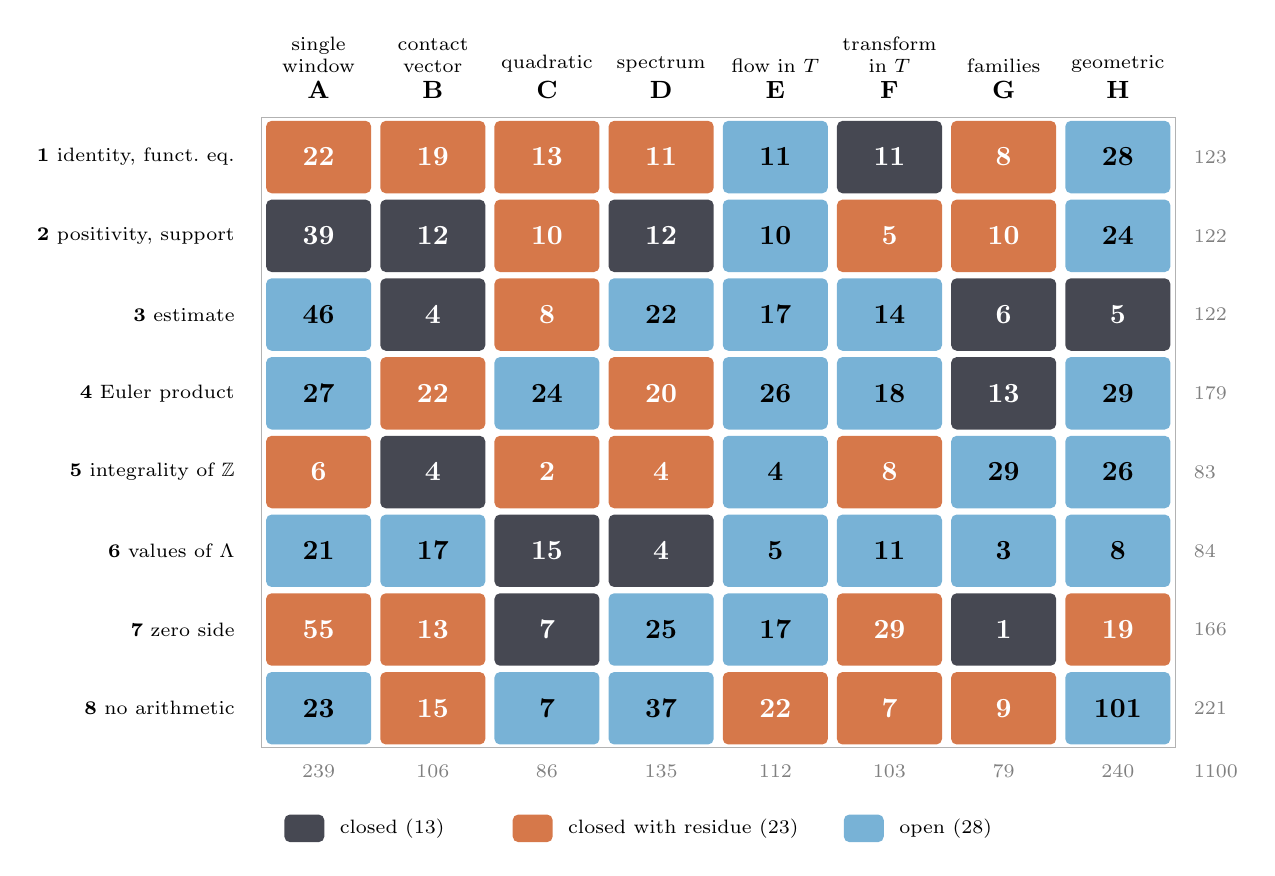
\begin{tikzpicture}[x=1.45cm,y=1.0cm,font=\small]
 \foreach \c/\lab [count=\i from 0] in {A/single window,B/contact vector,C/quadratic,D/spectrum,E/flow in $T$,F/transform in $T$,G/families,H/geometric}{
   \node[anchor=south] at (\i+0.5,0.12) {\textbf{\c}};
   \node[anchor=south,font=\scriptsize,text width=1.4cm,align=center] at (\i+0.5,0.45) {\lab};
 }
 \foreach \r/\lab [count=\j from 1] in {1/{identity, funct.\ eq.},2/{positivity, support},3/estimate,4/Euler product,5/integrality of $\Z$,6/values of $\Lambda$,7/zero side,8/no arithmetic}{
   \node[anchor=east,font=\scriptsize] at (-0.15,-\j+0.5) {\textbf{\r}\ \lab};
 }
 \foreach \row [count=\j from 1] in {
   {R/22,R/19,R/13,R/11,O/11,P/11,R/8,O/28},
   {P/39,P/12,R/10,P/12,O/10,R/5,R/10,O/24},
   {O/46,P/4,R/8,O/22,O/17,O/14,P/6,P/5},
   {O/27,R/22,O/24,R/20,O/26,O/18,P/13,O/29},
   {R/6,P/4,R/2,R/4,O/4,R/8,O/29,O/26},
   {O/21,O/17,P/15,P/4,O/5,O/11,O/3,O/8},
   {R/55,R/13,P/7,O/25,O/17,R/29,P/1,R/19},
   {O/23,R/15,O/7,O/37,R/22,R/7,R/9,O/101}}{
   \foreach \s/\n [count=\i from 0] in \row {
     \if\s P\def\fc{cDead}\def\tc{white}\fi
     \if\s R\def\fc{cRes}\def\tc{white}\fi
     \if\s O\def\fc{cOpen}\def\tc{black}\fi
     \fill[\fc,rounded corners=2pt] (\i+0.04,-\j+0.04) rectangle (\i+0.96,-\j+0.96);
     \node[text=\tc,font=\bfseries] at (\i+0.5,-\j+0.5) {\n};
   }
 }
 \draw[gray!60,line width=0.3pt] (0,0) rectangle (8,-8);
 \foreach \t [count=\i from 0] in {239,106,86,135,112,103,79,240}
   \node[font=\scriptsize,gray] at (\i+0.5,-8.3) {\t};
 \foreach \t [count=\j from 1] in {123,122,122,179,83,84,166,221}
   \node[font=\scriptsize,gray,anchor=west] at (8.08,-\j+0.5) {\t};
 \node[font=\scriptsize,gray,anchor=west] at (8.08,-8.3) {1100};
 \begin{scope}[shift={(0.2,-9.2)}]
   \fill[cDead,rounded corners=2pt] (0,0) rectangle (0.35,0.35); \node[anchor=west,font=\scriptsize] at (0.4,0.17) {closed (13)};
   \fill[cRes,rounded corners=2pt] (2.0,0) rectangle (2.35,0.35); \node[anchor=west,font=\scriptsize] at (2.4,0.17) {closed with residue (23)};
   \fill[cOpen,rounded corners=2pt] (4.9,0) rectangle (5.25,0.35); \node[anchor=west,font=\scriptsize] at (5.3,0.17) {open (28)};
 \end{scope}
\end{tikzpicture}
\caption{The $8\times8$ grid of routes. Rows: the $\zeta$-specific datum used at the sign step; columns: the carrying object. The
number is the number of routes in the cell; margins are totals. No cell is empty.}
\label{fig:grid}
\end{figure}

Three features stand out. Row 2 (positivity and support) is closed in columns A, B, D: deletion and amplification kill everything
that uses only $a\ge0$ and prime support. Column G is closed in rows 3, 4, 7 by the method theorems and the rationality wall. The
open cells concentrate in rows 4--8 and columns A, E, H, and most open entries there are unbuilt objects; row 6, the exact values
of $\Lambda$, has only ever been used linearly, where $\Lambda*1=\log$ acts as a window translation $T\mapsto T+\frac12\log X$ or
cancels at composite thresholds.

The tables that follow give, for each family, the idea, where it fails, and the status. Labels refer to the conclusion about
the route, not to the tools it produced.

\subsection{Classical and early families}
\begin{longtable}{@{}L{3.3cm}L{5.0cm}L{4.4cm}L{1.6cm}@{}}
\caption{Classical families.}\label{tab:classical}\\
\toprule
family & idea & where it fails & status \\
\midrule\endfirsthead
\toprule family & idea & where it fails & status\\ \midrule\endhead
\bottomrule\endfoot
statistics of Dirichlet polynomials & resonance, $\omega$-classes, extreme values, classifiers & numerical only; ``multiplicativity suppresses resonance'' refuted by the Liouville function & dead \\
inverse spectral, Hilbert--P\'olya, Jacobi, Mercer & realize the form as a positive operator & postulates the positivity (carrier absent) & no-go \\
Li--Keiper coefficients, Bochner kernels on ordinates & positivity of a sequence or kernel & REF; blind to the real parts & REF \\
heat flow, de Bruijn--Newman, Laguerre--P\'olya, Jensen & a flow preserving positivity & dynamical no-go; circular; heat traces are window data & no-go \\
total positivity, P\'olya frequency, Sturm, nodal measures & sign-regularity of kernels & fails $\mathrm{PF}_2$ at windows; nodal counts satisfied by models & dead \\
Baker, linear forms in logarithms & Diophantine separation of $\log n$ & far too weak at resolution $e^{-2T}$ & dead \\
Kre\u{\i}n, de Branges, Herglotz & positivity of an extension problem & REF: indeterminacy at every window is row D & REF \\
Nyman--Beurling completeness & approximation & REF & REF \\
dual, lattice, flat-top, exterior certificates & certify each window & Theorem~\ref{thm:Z}: the certificate is the explicit formula; Theorem~\ref{thm:finZ}; lattice ceilings & REF / no-go \\
sums of squares & SOS of Dirichlet polynomials & Theorem~\ref{thm:sos}, $T\ge\frac12\log3$ & no-go \\
sieves, progressions, short intervals, BV, Brun--Titchmarsh & bound the comb & Theorem~\ref{thm:finmod}; $b_\theta$; sieves hold in Beurling systems with off-line zeros & no-go \\
zero information & zero-free regions, densities, verified zeros & Theorems~\ref{thm:finmod}, \ref{thm:finZ} & no-go \\
Dirichlet-character families & average over $\chi$ & Parseval extracts no fibre (T5) & no-go \\
function fields, Hodge, Arakelov, Deligne, Laumon, $\mathbb F_1$ & transport the Weil/Hodge proof & no $h^0$ with the required three properties, not even over $\mathbb F_q$ (frame defect \cite{Paper46}); rationality wall; the six-clause adelic object of \cite[\S28.4]{Paper46} unbuilt & no-go; residue \\
Euler/M\"obius operator algebra, cones and orders in the form & order the form by its factors & linear identities plus Bochner and Cauchy--Schwarz only; resolvent cone and relative orders falsified & no-go \\
$\sigma$-transport, reflection, Frobenius dilation & move positivity from $\Rel s>1$ & the odd factor is void; part $1<\sigma\le\frac32$ is a zero-free statement & no-go \\
integer-lattice matrices, near coincidences & $\mathrm{Arch}_M-\mathrm{Div}_M-\mathrm{Near}_M\succeq0$ & exact restatement; near-coincidence part open & REF; open (\S\ref{subsec:restate}) \\
height flow on $\Q_{>0}$ & organize by height & pointwise part is zero geometry & no-go \\
\end{longtable}

\subsection{First-contact and witness families}\label{subsec:witness}
If the complete form fails, let $T_c=\sup\{T:\lamW>0\}$ and $E_c=\ker W_{T_c}$. The following is proved in the record under that
hypothesis.

\begin{proposition}[structure at a complete first contact; record]\label{prop:witness}
(i) Moving a non-real zero $w$ of $\Fh$ to $\bar w$ preserves $\|F\|$, the support, the domain and $W_T$; this holds for every window
datum with real multiplier and conjugation-closed polar block. (ii) $E_c$ is finite-dimensional, its nonzero elements have convex
support $[-T_c,T_c]$, and each parity part contains a real witness whose transform has only real zeros, of density $T_c/\pi$.
(iii) For distinct real zeros $x\ne y$ of $\Fh$ the node tests $\Fh/(z-x)$ are $W_{T_c}$-orthogonal, and on their span
$W_{T_c}(G)=\sum_xw_x|\widehat G(x)|^2$ with $w_x\ge0$.
\end{proposition}

\begin{theorem}[the $\times p$ cocycle; proved]\label{thm:cocycle}
Let $\nu_d=\frac1d\sum_{r\bmod d}\delta_{r/d}$ on $\R/\Z$ and $\Phi_a=\sum_{d\ge2}a(d)(\nu_d-\Leb)$, so $\widehat{\Phi_a}(k)=(a*1)(|k|)$
for $k\ne0$. Let $(\cL_p\Phi)^\wedge(k)=\widehat\Phi(pk)$. Then $\cL_p\Phi_\Lambda-\Phi_\Lambda=\log p\,(\delta_0-\Leb)$ for every prime $p$;
conversely the identity for all $p$ forces $a=\Lambda$. For a Beurling system with integers not in $\Z$, $\Phi$ is not defined.
\end{theorem}
\begin{proof}
$\widehat{\Phi_\Lambda}(k)=\log|k|$ and $\log|pk|-\log|k|=\log p$; the converse is induction on the number of prime factors and
M\"obius inversion; $\nu_g$ requires $g\in\Z$.
\end{proof}

\begin{theorem}[positive-off-$\N$ rigidity; record, proved]\label{thm:Rid}
Let $f(s)=\int_{[1,\infty)}\lambda^{-s}dN(\lambda)$ with $N(\{1\})=1$. Suppose (a) $N=N_\zeta$ on $[1,X)$ for some $X>1$; (b) $N\ge0$ on
$[1,\infty)\setminus\N$; (c) $\pi^{-s/2}\Gamma(s/2)f$ has $\zeta$'s functional equation, its simple poles with its residues and finite
order. Then $f=\zeta$.
\end{theorem}
\begin{proof}
By the Hecke--Bochner dictionary the even measure $m=\delta_0+N+\check N$ is tempered and self-dual. Put $\eta=m-\sum_{n\in\Z}\delta_n$;
then $\widehat\eta=\eta$, $\eta=0$ on $(-X,X)$, and $\eta_-$ is carried by $\Z$. With $\psi=\mathbf 1_{[-1/2,1/2]}*\chi$, $\chi\in C_c^\infty(-a,a)$,
$a<\frac{X-1}2$, and $\varphi=\psi*\tilde\psi$, one gets $\int|\widehat\psi|^2d\eta=0$; $\widehat\psi$ vanishes on $\Z\setminus\{0\}$, so
$\eta_+$ is carried by $(\Z\setminus\{0\})\cup Z(\widehat\chi)$; modulating $\chi$ moves $Z(\widehat\chi)$, so $m$ is carried by $\Z$, hence
$1$-periodic in transform, hence the Dirac comb.
\end{proof}
Hamburger's theorem is the case $\supp N\subset\N$. Every global property in the record that separates $\zeta$ from all the falsifiers
identifies it, and the properties that do not identify do not separate (integer frequencies at conductor $q>1$ contain $f_\chi$;
on-line abundance is shared by Davenport--Heilbronn combinations \cite{BombieriHejhal1995}; a positive tail without the functional
equation is blind to the zeros). After identification the sign must still come from the values of $\Lambda$.

\begin{longtable}{@{}L{3.3cm}L{5.0cm}L{4.4cm}L{1.6cm}@{}}
\caption{First-contact and witness routes.}\label{tab:witness}\\
\toprule
route & idea & where it fails & status \\
\midrule\endfirsthead
\toprule route & idea & where it fails & status\\ \midrule\endhead
\bottomrule\endfoot
Gamma moments, ports, jets at the contact & linear functionals of the contact vector & enter as $\lambda\langle\cdot,\cdot\rangle$, vanish at $\lambda=0$ (F1); finite Poisson--Chebyshev identity is orientation-invariant (F2) & no-go \\
linear limits & renormalized finite identities & tautological completions (F4); general exclusion not claimed & dead \\
Blaschke--torsion pairing & pair $\Phi_\Lambda$ with a non-band-limited test built from the Gauss nodes & node tests are Paley--Wiener and read only the window comb; the node measure is the determinate extension (REF) & no-go; residue: a signed $Z'/Z$ at the nodes \\
Selberg difference channel & $\Lambda\log+\Lambda*\Lambda=\mu*\log^2$ at the edge & node quadrature exact on type $\le2T_c$: channel values are values of $W$; residue the parity of the witness, closed & no-go \\
$\times p$ rigidity, o-minimal counting & measure rigidity for $\Phi_\Lambda$ & node sets not definable; no variety attached; rationality wall & no-go \\
weak renormalisation limit & a global object in $T$ with Euler before regularisation & limit vanishes modulo Tate; radicality is the target & no-go \\
finite multiplicity of exceptional zeros & a class statement on the zero set & the finite models $M_m$ share every class-level property; inertia chain of $M_m$ is that of $\zeta$ plus finite rank & no-go \\
Gamma--Euler detector & $-\zeta'/\zeta(2m+1)$ & detects only Gamma moments; faithful comparison has norm $\gtrsim1/\lamA$ & no-go \\
identification by global properties & separate $\zeta$ from the falsifiers & Theorem~\ref{thm:Rid}: every separator identifies & no-go \\
spectral invariants at the witness & determinants, heat traces & window data only & dead \\
node jets & read the angle of an exceptional quartet at a node & the node weights are blind to it (jet hierarchy, proved) & no-go \\
drop-term inequalities & discard a signed tail & hold whatever the zeros are; need a lower bound that is the target & REF \\
interlacing & nodes interlace the zeros & interlacing at critical density does not exclude a quartet (explicit pair $\sin,\cos$) & dead \\
mechanisms by requirement & survey of about $230$ mechanisms: global in the nodes, beyond the window, not one explicit-formula test & none meets all three; ``(iii) implies (ii)'' proved & no-go \\
twisted Chebyshev at one scale & inequality $(\mathrm{WS}^*)$ & unreachable by sieves ($b_\theta$), circular with zeros & open as statement \\
\end{longtable}

\subsection{The Beurling frontier}\label{subsec:beurling}
A \emph{discrete} Beurling system has prime measure $\sum_j\sum_kk^{-1}\delta_{p_j^k}$ with integer multiplicities. These are statements
about Beurling systems only; as routes to row D they fail because the integer count does not see the window form.

\begin{theorem}[discrete Beurling frontier; record, proved]\label{thm:BFdisc}
For $\theta\in(\frac13,\frac12)$ there is, almost surely, a discrete Beurling system with integer multiplicities, $N(x)=\rho x+O(x^{\theta+\varepsilon})$,
whose zeta function continues to $\sigma>\frac{1-\theta}2$ with zeros exactly at $\theta+(1-\theta)\varrho$, $\varrho$ the nontrivial zeros
of $\zeta$; a positive proportion of them lie on $\Rel s=\frac{1+\theta}2$.
\end{theorem}
\begin{proof}[Sketch]
Rescale $\zeta$ to $\zeta_\theta(s)=\zeta((s-\theta)/(1-\theta))$ \cite[\S6.1]{Broucke2024}, write its Euler factors with necklace exponents
$c_k(p^a)$, $a=\theta/(1-\theta)$, and round them independently at random to integers. The perturbation $FG$ is a random multiplicative
function with independent mean-zero values at primes; its moments are bounded by an Euler product convergent exactly when $2a>1$, i.e.\
$\theta>\frac13$, which gives the counting error by Borel--Cantelli, and $\log G$ converges almost surely for $\Rel w>\frac12-a$.
\end{proof}
A deterministic specialization gives a computable system $P_{171}$ with $N=cx+O(x^{83/208})$ and infinitely many zeros on
$\Rel s=\frac{11}{16}$ (record, proved). The prior construction closest to this, \cite[Thm.~1.3]{BDR2023}, is conditional and lies outside
these parameters; \cite[Ch.~17]{DiamondZhang2016} has not been checked against it, and no priority is claimed. Further proved items: a
system with $N(x)=\lfloor x\rfloor+c$ eventually is $\N$; adding an Euler factor with nonnegative multiplicities creates no zeros to the
right of its abscissa, so no system with small error and off-line zeros arises that way; the linear rounding theorem is false (dithered
rounding beats the variance) while the full system returns to exponent $\frac{1-\theta}2$ (argued); in the relaxed class without
integrality the exponent can be beaten for $\theta<\frac15$, so integrality is indispensable. Open: a discrete system with $\theta<\frac13$ and a
zero with real part $>\frac12$.

\subsection{Sonin, operator and inertia families}
\begin{longtable}{@{}L{3.3cm}L{5.0cm}L{4.4cm}L{1.6cm}@{}}
\caption{Operator routes.}\label{tab:operator}\\
\toprule
route & idea & where it fails & status \\
\midrule\endfirsthead
\toprule route & idea & where it fails & status\\ \midrule\endhead
\bottomrule\endfoot
Sonin trace, Connes--Consani, prolate & positive part plus small remainder & Theorem~\ref{thm:opbarriers}(1): remainder has $n_-=\infty$ for $T>\frac12\log2$; a source-computed norm bound is blind, a form-defined one is REF & no-go \\
coercivity and Schur reduction & $\lamA>0\iff S_{T,k}\succ0$ & exact; carries the whole margin & REF; open \\
Wiener--Hopf pencil, Birman--Schwinger & sign of $1-\beta_1$ & determinants inherit the margin & no-go \\
Nyquist sampling, two sectors & the form reads the symbol on $\pi k/2T$ & coherence inequality equals the target & REF \\
polar capacity & $\mathfrak G_T\succ0$ & inverts the primitive form; monotone, but every use consumes $\lamA>0$ & REF \\
interlacing and first crossing for $S_{T,k}$ & continue in $T$ & $k$ counts blocks, not contacts; no rank-one border; Hellmann--Feynman at a crossing is a functional of the minimizer & no-go \\
Tate transfer system $2\times2$ & canonical system from the boosts & positive for every chain, identical for $M_m$ & no-go \\
boundary triples & self-adjoint realization & Tate triple is the polar capacity; hypothesis is $\lamA\ge0$ & REF \\
spectral flow, Maslov & crossing forms & tool only: turns non-crossing into the sign of a finite form at the crossing & tool \\
\end{longtable}

\subsection{Sign-object constructions}\label{subsec:signobject}
Five campaigns tried to build an object carrying the sign, after the barriers of \S\ref{sec:barriers} were known. Their common outcome is a
classification: every lower bound for $\lamA$ built from the inputs tried falls in one of five branches, (1) comb-generic, (2) REF or a
certificate, (3) a functional of the minimizer, (4) blind to $\zeta$, (5) an equality between data (proved branch by branch; exhaustiveness
argued). The composition rule once proposed for these branches is \emph{refuted} as a barrier: a conjunction of inputs with no common falsifier
escapes the transfer lemma (Proposition~\ref{prop:EFI}).

\begin{longtable}{@{}L{3.3cm}L{5.0cm}L{4.4cm}L{1.6cm}@{}}
\caption{Sign-object constructions.}\label{tab:signobject}\\
\toprule
object & idea & where it fails & status \\
\midrule\endfirsthead
\toprule object & idea & where it fails & status\\ \midrule\endhead
\bottomrule\endfoot
L\'evy structure, Hamburger rigidity & positivity from the L\'evy--Khintchine form & classical; rigidity identifies; REF & no-go \\
pair surface, Hodge index, Riemann--Roch & a surface whose Hodge index gives the sign & tautological ($\langle\Gamma_g,\Gamma_g\rangle=\mathfrak a_T$) & no-go \\
pair counts over $\N\times\N$, Farey, coprimality & an $h^0$ off the multiplicative diagonal & no measure on $\log\Q$ equals $\mathfrak a_T$ on $\PT$; limit identity is $\mathrm{Arch}-\mathrm{Near}$ & REF \\
cones through $\partial\log$ & carry positivity to $-\zeta'/\zeta$ & only infinitely divisible cones cross; homogeneous, killed by $c\Lambda$ & no-go \\
coefficient integrality, additive inputs, gauges & integrality or divisor gauges & Theorem~\ref{thm:scale}; gauges are comb-generic & no-go \\
reflection positivity at the edge & Osterwalder--Schrader at $x=T$ & reflection identity false; the gap protects products, the sign lives in quotients & no-go \\
$\Gamma$-limit, solenoid defect & limit objects & comb-generic; M\"obius is not a cocycle & no-go \\
quotient ladders, leakage quotient & coordinates after cancellation & tautological modulo the radical & no-go \\
Epstein defect cumulants & class-group cumulants of the Euler defect & finite indefinite comb on $\PT$ & no-go \\
free and exogenous variables & import a variable & Rankin, Hecke--Petersson, shifted Selberg: REF or gamma/conductor only & no-go \\
oscillation counts & sign changes & gap iff a cut foreign to the comb & no-go \\
nonnegative rank, sign rank & integer invariants of a slack matrix & block structure gives invariant $\equiv0$ for every comb (exact computation, 1080 matrices) & no-go \\
recurrence $\{x+y,xy\}$ & Ramsey-type recurrence & a function of finitely many data, locally constant & no-go \\
bound states, trace identities, pressure, transport & positivity of an auxiliary operator & local invariants are blind to atoms; positivity for every comb cannot equal the form & no-go \\
exterior table $(\star\star)$ & dominate the leakage on the exterior & signed Euler product on the exterior is the $1/\zeta$ channel; only identities & dead \\
concavity in the comb & Danskin derivative & gives only upper bounds; lower bounds only by chords & no-go \\
hierarchical ladder of contacts & each prime cancels the rest at its scale & the ladder is the edge profile of the minimizer, smooth in $\log n$, comb-generic & no-go \\
\end{longtable}

\subsection{Reformulations and their tractability}
Roughly $360$ routes of the record end in an internal reformulation. They reduce to $43$ distinct statements. Each was examined for a path of
its own, independent of row D, with general theorems applicable even if stronger. None has one: $22$ only transfer the positivity (a general
theory consumes the positivity of the window datum), $21$ do not. The hypotheses consumed are four: positivity at all windows, invertibility in
a sector or block, uniform control in $T$, and the prime tail. Constructions closed in this examination: interlacing for $S_{T,k}$; quadratic
operators $\mathfrak a_T=B^*B$ (Theorem~\ref{thm:sos} extends to arbitrary real frequencies, so no convolutive $B$ exists for $T\ge\frac12\log3$);
the polar capacity; the half-line convexity lemma (false, explicit counterexample with negative second derivative); exact Schur complements
coupling Euler and the gap (the coupling is null, the inputs chain); sign patterns of the minimizer (the extremal at $\frac12\log15$ is of one
sign; it is its M\"obius inverse that changes sign); the damped interpolation $(1-t)\rho_\kappa+t\Lambda$, whose threshold $t_\infty>0$ is
invariant under finite modifications and so does not imply row D. Their positive output is Theorem~\ref{thm:eveninertia} and
Theorem~\ref{thm:archcount}.

\subsection{Composing the Euler product and the functional equation}\label{subsec:compose}
\begin{longtable}{@{}L{3.3cm}L{5.0cm}L{4.4cm}L{1.6cm}@{}}
\caption{Attempts to compose (E) and (F) in one sign step.}\label{tab:compose}\\
\toprule
attempt & idea & where it fails & status \\
\midrule\endfirsthead
\toprule attempt & idea & where it fails & status\\ \midrule\endhead
\bottomrule\endfoot
functional equation as a symmetry of the polar vector & use (F) through $h_{\mathrm{par}}$ & (F) leaves in the window form only weight-independent traces; chains & no-go \\
Euler defect with a seminorm & $2\delta_E(\Lambda;f)^2=\ell(Ef)$ & (E) enters as an identity, (F) as a fixed seminorm & no-go \\
skeleton of the mechanism & \S\ref{subsec:mechanism} & four steps proved; no sign node; high-frequency failure of the polar control & open (node) \\
reciprocity objects: Hecke, Weil, Hamburger, theta, Eisenstein, Rankin--Selberg, Voronoi, Kuznetsov, Estermann, Kronecker--Hurwitz & quadratic version of the rigidity & Voronoi with $|g|^2$ holds for Epstein; Kuznetsov reads $\zeta$ only at abscissa $1$; large-sieve positivity is a generic norm; quadratic rigidity is a generic norm plus an identity & no-go \\
class impossibility for the node & one theorem for continuous steps & is the total-variation theorem (Theorem~\ref{thm:geotv}) plus $a_P$; the finite-block version is conditional on an open approximation statement & cited \\
determinants or moments of order $T$ & amplify sensitivity & already excluded (Theorem~\ref{thm:opbarriers}(2)) & no-go \\
weight-$\frac12$ forms with native functional equation & \S\ref{subsec:emptycell} & principal part trivial or without mechanism, outside the node's band & no-go \\
zero-side certificate of the node & verified zeros & valid at grid points to $4.245$; a verification, not a mechanism & tool \\
\end{longtable}

%=====================================================================
\section{What is open}\label{sec:open}

\subsection{The node}
For $F$ real and even in the form domain on $[-T,T]$ put
\[
\ell_T(F)=\int F(x)\cosh\tfrac x2\,dx,\qquad \Phi_T(F)=-\int_{[1^-,e^{2T}]}2t^{-1/2}c_F(\log t)\,d\big(\psi(t)-t\big),
\]
with $\eT$ as in \eqref{eq:eT}. On $\ell_T(F)=0$ one has, exactly, $(\mT+\eT)(F)+\Phi_T(F)=\mathfrak a_T(F)=W_T(F)$ (proved).

\begin{problem}[the node; open]\label{prob:node}
Prove that for every $T>\frac12\log15$ and every real even $F$ in the form domain with $\ell_T(F)=0$,
\[
Q_T(F):=(\mT+\eT)(F)+\Phi_T(F)\ \ge\ 0 .
\]
\end{problem}

The node carries three quantifiers, none of which can be dropped without a further theorem.
\emph{All modes:} its restriction to $E_N^{\mathrm{ev}}\cap c^\perp$, $N\approx4T$, is a compression; by min--max its bottom there is
$\ge$ the true bottom, so a bound on the block does not control the complement or the coupling.
\emph{All windows:} the zero-side certificate covers grid points of $[0.75,4.245]$ on the block, not the continuum, and fails from $4.25$ on
by loss of margin, not of sign.
\emph{The declared sector:} the node is the even sector without the polar term; a statement for row D must also treat the odd sector and the
polar term (Theorem~\ref{thm:eveninertia}(ii)).
Status: proved for $T\le\frac12\log5$ (from the certified complete form) and, granting \cite{Mori15}, for $T\le\frac12\log15$. The
first case with content is $T=\frac12\log5$ on $\{e_1,e_3\}$: numerically $(\mT+\eT)=-0.18913$, $\Phi=+0.19098$, the prime $2$ paying
$+0.510$ by the phase $\omega_3\log2\approx1.29\pi$, $a_P$ giving $-0.477$, and $c\Lambda$ failing below $c\approx0.9924$; with three modes the
margin falls to $10^{-6}$--$10^{-7}$. The node is a linear matrix inequality in the weights: its feasible set is a spectrahedron in
$(v_n)_{n<e^{2T}}$.

\subsection{Exact restatements of row D}\label{subsec:restate}
Each of the following is equivalent to row D (at the window or over all windows) by a theorem of \cite{Paper47}; each is open and a valid
target.
\begin{enumerate}
\item[(L2)] \emph{The finite matrix.} $S_{T,k(T)}\succeq0$, the Schur complement of $\mathfrak a_T$ on the $(2k-2)$-dimensional space of
piecewise Tate exponentials, $k\ge k_0(T)$; first case $T=\frac12\log5+\varepsilon$.
\item[(N)] \emph{Signed twisted Chebyshev bound at Nyquist points.} A pointwise bound with sign for the coherence of the comb at
$\omega_k=\pi k/2T$, correlated with the samples $|\Fh(\omega_k)|^2$; equivalently $\mathcal F_T\le\mathfrak a^\sharp$ on $\PT$ with archimedean
symbol $\Rel\psi(\frac54+\frac{i\tau}2)-\log\pi$. Absolute bounds for $\psi(y)-y$ with any exponent $>\frac12$ and mean-square bounds do not suffice.
\item[(S)] \emph{Near coincidences.} $\mathrm{Arch}_M-\mathrm{Div}_M-\mathrm{Near}_M\succeq0$ for every $M$, at a fixed profile with
$2T_0<\log2$; positivity holds on test spaces blind to near coincidences $m\approx kn$, $m\ne kn$.
\item[(L)] \emph{Leakage coercivity.} $W_T(g)\ge\kappa N^{-A_0}\ell(g)$ with the gauge-minimized leakage $\ell$, equivalently the exterior
inequality $(\star\star)$ on the aliasing tail \cite[Problem `leakage coercivity']{Paper47}.
\item[(1P)] \emph{One profile.} Positive definiteness of one explicit function of one real variable.
\end{enumerate}

\subsection{Statements weaker in appearance}
\begin{itemize}
\item $(\Omega_0)$: for every $T>\frac12\log5$, $\sum_n2\Lambda(n)n^{-1/2}h_T(\log n)<0$ for the clamped ground mode $h_T$ of $\PT$; necessary,
not sufficient.
\item $(E_\gamma)$: $\limsup_T\mathcal F_T(F_T)/\|F_T\|^2\le\Rel\psi(\frac54+\frac{i\gamma}2)-\log\pi$ for concentrating packets at one frequency;
implied by row D and exactly critical at every $\gamma$.
\item $(\Omega_{t_0})$: positivity along $(1-t)\rho_\kappa+t\Lambda$ up to a fixed fraction $t_\infty>0$; implied by row D, invariant under
finite modifications; whether strictly weaker is open.
\item The lower half of a two-sided law $\lamA=L(T)(1+o(1))$, $L>0$; any admissible $L$ is below Theorem~\ref{thm:margin}.
\item A non-linear multiscale inequality on $\Lambda$ outside single tests and power families (where it is circular, proved).
\item The six-clause adelic object of \cite[\S28.4]{Paper46}, the only path that reopens the Hodge-type programme.
\item An inequality at $\sigma=1$ using the multiplicativity of $\zeta$ on the line, false for $\zeta R$ with $R$ rational and for
Epstein and Davenport--Heilbronn series, and not a zero-free statement.
\item Arithmetic squares on $(\frac12\log2,\frac12\log3)$; a certified window beyond $\frac12\log5$ with $\mathfrak G_T\succ0$ by our own
methods.
\end{itemize}

\subsection{The empty cell}\label{subsec:emptycell}
In the literature surveyed, every built-in positivity reads the primes with weight at most $n^{-1}$ or lacks the functional equation:
Helson's multiplicative Hilbert matrix \cite{Helson2006} has weight $n^{-1/2}$ and no functional equation; automorphic norms have the functional equation
and weight $n^{-1}$. The cell ``weight $n^{-1/2}$, global functional equation, built-in positivity'' is empty. One attempt to fill it
uses the unitary involution $Jf(t)=\chi(\frac12+it)f(-t)$ on the critical line: by Gonek's stationary-phase lemma \cite{Gonek1984} the $J$-part of every
weight-$\frac12$ form is a multiplicative Hankel form $\sum_Nw(2\pi N)(a*a)(N)$. With $a=\Lambda$ and $w\ge0$ it is nonnegative
trivially and inherited by $a_P$ and $c\Lambda$ (no-go); with $w$ indefinite there is no mechanism, and its principal part lives at
heights $t\ge8\pi$, outside the band $|\tau|\lesssim2\pi$ of the node (argued). The compression to the node window is not $J$-stable,
since $\chi(\frac12+it)$ is not a multiplier of the Paley--Wiener space (proved).

\subsection{The live gate}
Combining Theorems~\ref{thm:aP} and \ref{thm:geotv}: a premise that holds for every Euler product with a pole fails the node for
$T>\pi/2$, and a premise robust in total variation has radius at most the margin. What neither excludes is a premise that is a theorem
\emph{only} for logarithmic derivatives of $L$-functions with an Euler product over all primes, not inherited by $a_P$, used with
precision at most $4\cdot10^9Te^{-15.449T}$, and leading to Problem~\ref{prob:node} for every $T$. No candidate is known. A proposal
must write the object, prove its positivity, and prove its exact link with $Q_T$; characterizing $\Lambda$ without that link gives no sign.

\appendix
\section{Sources in the research record}\label{app:index}
Identifiers $\mathrm Rn\_k$ are memos of phase $n$ of the author's research record; ``P$k$'' is Paper $k$.

\begin{center}\small
\begin{tabularx}{\textwidth}{@{}L{5.2cm}Y@{}}
\toprule
statement & record \\
\midrule
grid, counts, killer codes & R162\_2300 master grid (part 19, 1100 routes) \\
routes index, families, residues & ROUTES-TRIED-INDEX (README, 06\_OPEN\_RESIDUES); crossword CROSSWORD-TO-D \\
$n_-(\mT+\eT)\ge N'(T)$ & phase 205, SKELETON\_002 \\
zero-side reading \eqref{eq:zeroside}, signature $(1,1)$ & phase 204 H1PLUS\_001; phase 207 AUDIT\_207\_001 \\
mechanism in four steps, node, Stieltjes form & phase 206 README, NODE\_001, AUDIT\_206\_001 \\
node scope, three quantifiers, separators $b^{(p)}$ & phase 208 README \\
withdrawal of the doubly exponential margin & index correction after the shape theorem of P47 \\
certified battery & phase 198 CERT\_FALSIFIERS\_001; phase 200 MAP\_200\_001, CERT\_DH\_001 \\
five branches, composition refuted & phase 200 MAP\_200\_001; phase 204 O1\_COMPOSITION\_001 \\
untried families & phase 201 FAMILIES\_A/B/C, V1\_1\_NONNEG\_001, V2\_RECURRENCE\_001, CPOS\_CLASS\_001 \\
exterior table, concavity, ladder & phases 202--203 BUILD\_R1/R2, INVENT\_001, AUDIT\_203\_001 \\
reformulation tractability & phase 204 TRACT\_*, FINAL\_204\_001, WEAKEN\_001, P1\_BBSTAR\_001, LEMMA\_F\_HALFLINE\_001 \\
composition attempts & phase 204 COMPOSE\_EF\_001, AUDIT\_204\_CSTAR\_001; phase 206 RIGID\_001; phase 207 CLASS\_001, CELL\_001 \\
witness structure, cocycle & R160\_X\_C1; R162\_1001 \\
first-contact problems & R162\_2201--2602 \\
Theorem~\ref{thm:Rid}, identification & R164\_401, R164\_190; R163\_1001 \\
Theorem~\ref{thm:BFdisc}, $P_{171}$, Beurling items & R163\_803, R163\_891; R171\_FINAL; R184\_004--015 \\
witness routes, jets, $(\mathrm{WS}^*)$ & R164\_501--601, R165\_101--202, R166\_201, R166\_501, R166\_802, R167\_101--103 \\
Sonin, operator routes & R183\_018--033, R184\_015; phase 204 L2\_INTERLACE\_001, POLAR\_CAP\_001 \\
\bottomrule
\end{tabularx}
\end{center}

\begin{thebibliography}{99}
\bibitem{BDR2023} F.~Broucke, G.~Debruyne and Sz.~Gy.~R\'ev\'esz, \emph{Some examples of well-behaved Beurling number systems}, arXiv:2309.01567 (2023).
\bibitem{BombieriHejhal1995} E.~Bombieri and D.~A.~Hejhal, \emph{On the distribution of zeros of linear combinations of Euler products}, Duke Math.~J.\ \textbf{80} (1995), 821--862.
\bibitem{Bombieri2000} E.~Bombieri, \emph{Remarks on Weil's quadratic functional in the theory of prime numbers, I}, Atti Accad.~Naz.~Lincei Cl.~Sci.~Fis.~Mat.~Natur.~Rend.~Lincei (9) Mat.~Appl.\ \textbf{11} (2000), 183--233.
\bibitem{Broucke2024} F.~Broucke, \emph{On zero-density estimates for Beurling zeta functions}, arXiv:2409.10051 (2024).
\bibitem{ConnesConsani2021} A.~Connes and C.~Consani, \emph{Weil positivity and trace formula, the archimedean place}, Selecta Math.\ (N.S.) \textbf{27} (2021), Paper No.~77.
\bibitem{DiamondZhang2016} H.~G.~Diamond and W.-B.~Zhang, \emph{Beurling Generalized Numbers}, Math.\ Surveys Monogr.\ \textbf{213}, Amer.\ Math.\ Soc., 2016.
\bibitem{DMV2006} H.~G.~Diamond, H.~L.~Montgomery and U.~M.~A.~Vorhauer, \emph{Beurling primes with large oscillation}, Math.~Ann.\ \textbf{334} (2006), 1--36.
\bibitem{Gonek1984} S.~M.~Gonek, \emph{Mean values of the Riemann zeta function and its derivatives}, Invent.\ Math.\ \textbf{75} (1984), 123--141.
\bibitem{Helson2006} H.~Helson, \emph{Hankel forms and sums of random variables}, Studia Math.\ \textbf{176} (2006), 85--92.
\bibitem{Hamburger1921} H.~Hamburger, \emph{\"Uber die Riemannsche Funktionalgleichung der $\zeta$-Funktion}, Math.\ Z.\ \textbf{10} (1921), 240--254.
\bibitem{KaczorowskiKulas2007} J.~Kaczorowski and M.~Kulas, \emph{On the non-trivial zeros off the critical line for $L$-functions from the extended Selberg class}, Monatsh.\ Math.\ \textbf{150} (2007).
\bibitem{Liu2026} V.~Liu, \emph{Certified Weil positivity beyond the unit window: source-exact block-Schur and tail-compensation bounds for the Riemann zeta function}, manuscript, alphaXiv, under review at Math.\ Comp.\ (unrefereed).
\bibitem{Mori15} R.~Mori, \emph{Weil positivity on the window of width $\log 15$}, Zenodo (2026), doi:\nolinkurl{10.5281/zenodo.23281236} (unrefereed).
\bibitem{MoriUpper} R.~Mori, \emph{Improved upper bounds for windowed Weil forms with exponential factor $e^{-4\pi\mu}$}, Zenodo (2026), doi:\nolinkurl{10.5281/zenodo.23363767} (unrefereed).
\bibitem{Paper43} D.~A.~Trejo Pizzo, \emph{A correspondence algebra with a canonical trace on the idele class group}, preprint, 2026.
\bibitem{Paper44} D.~A.~Trejo Pizzo, \emph{An arithmetic Frobenius family and its integral shadow}, preprint, 2026.
\bibitem{Paper45} D.~A.~Trejo Pizzo, \emph{An explicit formula and a comparison theorem for the canonical trace on a correspondence algebra of the idele class group}, preprint, 2026.
\bibitem{Paper46} D.~A.~Trejo Pizzo, \emph{Row D: the sign}, preprint, 2026.
\bibitem{Paper47} D.~A.~Trejo Pizzo, \emph{Weil positivity on a finite window: duality, certificates and a finite reduction}, preprint, 2026.
\bibitem{SaiasWeingartner2009} E.~Saias and A.~Weingartner, \emph{Zeros of Dirichlet series with periodic coefficients}, Acta Arith.\ \textbf{140} (2009).
\bibitem{Weil52} A.~Weil, \emph{Sur les ``formules explicites'' de la th\'eorie des nombres premiers}, Comm.~S\'em.~Math.~Univ.~Lund (1952), 252--265.
\bibitem{Yoshida1992} H.~Yoshida, \emph{On Hermitian forms attached to zeta functions}, in: \emph{Zeta Functions in Geometry}, Adv.~Stud.~Pure Math.~\textbf{21}, Kinokuniya, Tokyo, 1992, 281--325.
\bibitem{Zhang2007} W.-B.~Zhang, \emph{Beurling primes with RH and Beurling primes with large oscillation}, Math.~Ann.\ \textbf{337} (2007), 671--704.
\bibitem{Zhu2026} X.~Zhu, \emph{Weil positivity in compact windows: a finite reduction, certified two-sided bounds, and a Landau--Widom decay law}, arXiv:2608.24827 (2026).
\end{thebibliography}

\end{document}
